\documentclass[aspectratio=169, professionalfonts]{beamer}

\usetheme{Szeged}
\usecolortheme{dolphin}

\usepackage{amsmath, amssymb, bm}
\usepackage{tikz}
\usetikzlibrary{positioning, arrows.meta, decorations.pathreplacing, calc}
\usepackage{pgfplots}
\pgfplotsset{compat=1.18}

\def\R{\mathbb{R}}
\def\E{\mathbb{E}}
\def\Var{\text{Var}}
\def\Cov{\text{Cov}}
\def\Bias{\text{Bias}}
\def\MSE{\text{MSE}}
\newcommand{\rank}{\operatorname{rank}}

\definecolor{mantis}{RGB}{0, 105, 62}

\setbeamercolor{frametitle}{fg=white, bg=mantis}
\setbeamercolor{title}{fg=white, bg=mantis}
\setbeamercolor{structure}{fg=mantis}
\setbeamercolor{block title}{bg=mantis, fg=white}
\setbeamercolor{block body}{bg=mantis!10}

\title{Mathematical Prerequisites}
\subtitle{Calculus, Linear Algebra, Probability \& Statistics}
\author{Lebnet Tech Fellows Program}
\date{}

\begin{document}

% ------------------------------------------------------------------
\begin{frame}
\titlepage
\end{frame}

% ------------------------------------------------------------------
\begin{frame}{Roadmap}
\tableofcontents
\end{frame}

% ==================================================================
\section{Calculus}
% ==================================================================

% ------------------------------------------------------------------
\begin{frame}{Derivatives and the Chain Rule}

The derivative $f'(x)$ is the slope of the tangent line at $x$:
$$f'(x) = \lim_{h \to 0} \frac{f(x+h) - f(x)}{h}$$

\bigskip

\textbf{Standard rules} (for differentiable $f, g$):
\begin{itemize}
  \item $(f + g)' = f' + g'$; \quad $(fg)' = f'g + fg'$; \quad $(f/g)' = (f'g - fg')/g^2$
  \item $(x^n)' = nx^{n-1}$; \quad $(e^x)' = e^x$; \quad $(\ln x)' = 1/x$
\end{itemize}

\bigskip

\begin{alertblock}{Chain Rule}
$(f \circ g)'(x) = f'(g(x)) \cdot g'(x)$
\end{alertblock}

Backpropagation in neural networks is the chain rule applied to a composition of many functions.

\end{frame}

% ------------------------------------------------------------------
\begin{frame}{Integration}

The integral $\int_a^b f(x)\,dx$ is the signed area under $f$:

$$\underbrace{\sum_{i=1}^{n} f(x_i)\,\Delta x}_{\text{Riemann sum}} \;\xrightarrow[\Delta x \to 0]{n \to \infty}\; \underbrace{\int_a^b f(x)\,dx}_{\text{exact area}}$$

\bigskip

\begin{block}{Fundamental Theorem of Calculus}
If $F'(x) = f(x)$, then $\displaystyle\int_a^b f(x)\,dx = F(b) - F(a)$.
\end{block}

\bigskip

Differentiation and integration are inverse operations. This duality appears in the relationship between the PDF and CDF.

\end{frame}

% ------------------------------------------------------------------
\begin{frame}{Partial Derivatives and the Gradient}

For $f : \R^d \to \R$, the partial derivative $\frac{\partial f}{\partial x_j}$ measures the rate of change along the $j$-th axis (others held fixed).

\bigskip

The \textbf{gradient} collects all partial derivatives:
$$\nabla f(\mathbf{x}) = \begin{bmatrix} \frac{\partial f}{\partial x_1} \\ \vdots \\ \frac{\partial f}{\partial x_d} \end{bmatrix} \in \R^d$$

\bigskip

\begin{itemize}
  \item $\nabla f(\mathbf{x})$ points in the direction of \textbf{steepest ascent}
  \item $\|\nabla f\|$ is the rate of increase in that direction
  \item On a contour plot, $\nabla f$ is $\perp$ to level curves
  \item \textbf{Gradient descent:} step in $-\nabla f$ to decrease $f$ as fast as possible
\end{itemize}

\end{frame}

% ------------------------------------------------------------------
\begin{frame}{Critical Points, Hessian, and Convexity}

At a critical point $\nabla f(\mathbf{x}^*) = \mathbf{0}$, use the \textbf{Hessian} $\mathbf{H}_f = [\partial^2 f / \partial x_i \partial x_j]$ to classify:

\begin{itemize}
  \item $\mathbf{H}_f \succ 0$ (all $\lambda > 0$): local minimum
  \item $\mathbf{H}_f \prec 0$ (all $\lambda < 0$): local maximum
  \item Otherwise: saddle point
\end{itemize}

\bigskip

\begin{block}{Convexity}
$f$ is \textbf{convex} if $\mathbf{H}_f(\mathbf{x}) \succeq 0$ everywhere, equivalently:
$$f(t\mathbf{a} + (1-t)\mathbf{b}) \leq t\,f(\mathbf{a}) + (1-t)\,f(\mathbf{b}) \quad \forall\, \mathbf{a}, \mathbf{b},\; t \in [0,1]$$
For convex $f$, every local minimum is a \textbf{global} minimum.
\end{block}

\bigskip

OLS loss is convex $\Rightarrow$ unique solution. Neural network loss is non-convex $\Rightarrow$ no such guarantee.

\end{frame}

% ==================================================================
\section{Linear Algebra}
% ==================================================================

% ------------------------------------------------------------------
\begin{frame}{Matrices as Linear Transformations}

A matrix $\mathbf{A} \in \R^{m \times n}$ defines $f(\mathbf{x}) = \mathbf{A}\mathbf{x}$.

\bigskip

The $j$-th column of $\mathbf{A}$ is the image of $\mathbf{e}_j$. For any $\mathbf{x}$:
$$\mathbf{A}\mathbf{x} = x_1\,(\mathbf{A}\mathbf{e}_1) + x_2\,(\mathbf{A}\mathbf{e}_2) + \cdots + x_n\,(\mathbf{A}\mathbf{e}_n)$$

\begin{center}
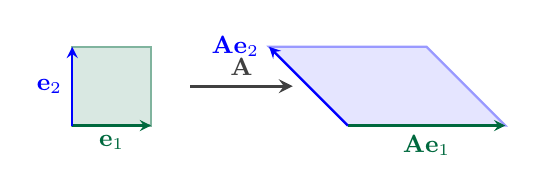
\begin{tikzpicture}[>=stealth, scale=1.0]
    \fill[mantis!15] (0,0) -- (1,0) -- (1,1) -- (0,1) -- cycle;
    \draw[thick, mantis!50] (0,0) -- (1,0) -- (1,1) -- (0,1) -- cycle;
    \draw[->, thick, mantis] (0,0) -- (1,0) node[midway, below, font=\small] {$\mathbf{e}_1$};
    \draw[->, thick, blue] (0,0) -- (0,1) node[midway, left, font=\small] {$\mathbf{e}_2$};
    \draw[->, very thick, darkgray] (1.5, 0.5) -- node[above, font=\small] {$\mathbf{A}$} (2.8, 0.5);
    \begin{scope}[shift={(3.5,0)}]
    \fill[blue!10] (0,0) -- (2,0) -- (1,1) -- (-1,1) -- cycle;
    \draw[thick, blue!40] (0,0) -- (2,0) -- (1,1) -- (-1,1) -- cycle;
    \draw[->, thick, mantis] (0,0) -- (2,0) node[midway, below, font=\small] {$\mathbf{A}\mathbf{e}_1$};
    \draw[->, thick, blue] (0,0) -- (-1,1) node[left, font=\small] {$\mathbf{A}\mathbf{e}_2$};
    \end{scope}
\end{tikzpicture}
\end{center}

The unit square maps to a parallelogram spanned by the columns of $\mathbf{A}$. A linear transformation can scale, rotate, reflect, shear --- but cannot bend or warp.

\end{frame}

% ------------------------------------------------------------------
\begin{frame}{Types of Transformations}

\begin{center}
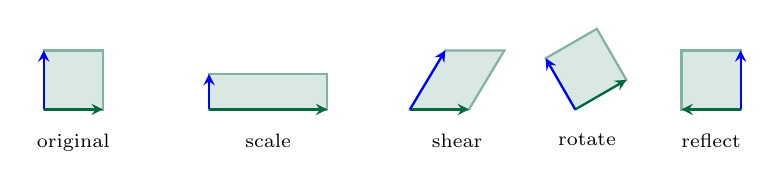
\begin{tikzpicture}[>=stealth, scale=0.75]
\begin{scope}[shift={(0,0)}]
    \fill[mantis!15] (0,0) -- (1,0) -- (1,1) -- (0,1) -- cycle;
    \draw[thick, mantis!50] (0,0) -- (1,0) -- (1,1) -- (0,1) -- cycle;
    \draw[->, thick, mantis] (0,0) -- (1,0);
    \draw[->, thick, blue] (0,0) -- (0,1);
    \node[below, font=\scriptsize] at (0.5,-0.25) {original};
\end{scope}
\begin{scope}[shift={(2.8,0)}]
    \fill[mantis!15] (0,0) -- (2,0) -- (2,0.6) -- (0,0.6) -- cycle;
    \draw[thick, mantis!50] (0,0) -- (2,0) -- (2,0.6) -- (0,0.6) -- cycle;
    \draw[->, thick, mantis] (0,0) -- (2,0);
    \draw[->, thick, blue] (0,0) -- (0,0.6);
    \node[below, font=\scriptsize] at (1,-0.25) {scale};
\end{scope}
\begin{scope}[shift={(6.2,0)}]
    \fill[mantis!15] (0,0) -- (1,0) -- (1.6,1) -- (0.6,1) -- cycle;
    \draw[thick, mantis!50] (0,0) -- (1,0) -- (1.6,1) -- (0.6,1) -- cycle;
    \draw[->, thick, mantis] (0,0) -- (1,0);
    \draw[->, thick, blue] (0,0) -- (0.6,1);
    \node[below, font=\scriptsize] at (0.8,-0.25) {shear};
\end{scope}
\begin{scope}[shift={(9.0,0)}]
    \fill[mantis!15] (0,0) -- (0.866,0.5) -- (0.366,1.366) -- (-0.5,0.866) -- cycle;
    \draw[thick, mantis!50] (0,0) -- (0.866,0.5) -- (0.366,1.366) -- (-0.5,0.866) -- cycle;
    \draw[->, thick, mantis] (0,0) -- (0.866,0.5);
    \draw[->, thick, blue] (0,0) -- (-0.5,0.866);
    \node[below, font=\scriptsize] at (0.2,-0.25) {rotate};
\end{scope}
\begin{scope}[shift={(11.8,0)}]
    \fill[mantis!15] (0,0) -- (-1,0) -- (-1,1) -- (0,1) -- cycle;
    \draw[thick, mantis!50] (0,0) -- (-1,0) -- (-1,1) -- (0,1) -- cycle;
    \draw[->, thick, mantis] (0,0) -- (-1,0);
    \draw[->, thick, blue] (0,0) -- (0,1);
    \node[below, font=\scriptsize] at (-0.5,-0.25) {reflect};
\end{scope}
\end{tikzpicture}
\end{center}

\begin{itemize}
  \item \textbf{Diagonal:} scale each axis independently; identity is the special case
  \item \textbf{Shear:} off-diagonal entries tilt the square into a parallelogram
  \item \textbf{Rotation:} $\mathbf{R}_\theta = \begin{bmatrix}\cos\theta & -\sin\theta \\ \sin\theta & \cos\theta\end{bmatrix}$; preserves lengths and angles
  \item \textbf{Composition:} $\mathbf{A}\mathbf{B}$ applies $\mathbf{B}$ first, then $\mathbf{A}$; generally $\mathbf{A}\mathbf{B} \neq \mathbf{B}\mathbf{A}$
  \item \textbf{SVD:} any matrix $=$ rotation $\times$ scaling $\times$ rotation
\end{itemize}

\end{frame}

% ------------------------------------------------------------------
\begin{frame}{The Dot Product}

Two equivalent definitions for $\mathbf{x}, \mathbf{y} \in \R^d$:
$$\mathbf{x}^\top\mathbf{y} = \sum_{i=1}^{d} x_i y_i = \|\mathbf{x}\|\,\|\mathbf{y}\|\cos\theta$$

\begin{center}
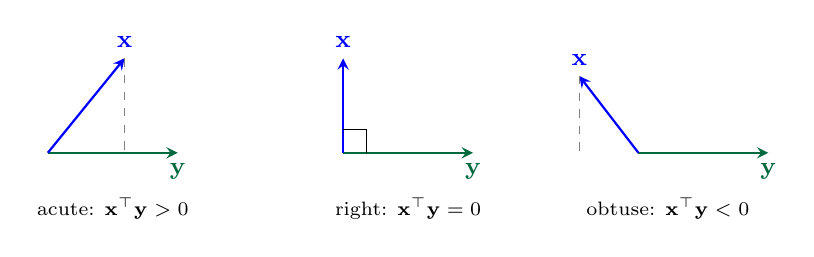
\begin{tikzpicture}[>=stealth, scale=0.75]
\begin{scope}[shift={(0,0)}]
    \draw[->, thick, mantis] (0,0) -- (2.2,0) node[below, font=\small] {$\mathbf{y}$};
    \draw[->, thick, blue] (0,0) -- (1.3,1.6) node[above, font=\small] {$\mathbf{x}$};
    \draw[dashed, gray] (1.3,1.6) -- (1.3,0);
    \node[below, font=\scriptsize] at (1.1,-0.6) {acute: $\mathbf{x}^\top\mathbf{y} > 0$};
\end{scope}
\begin{scope}[shift={(5,0)}]
    \draw[->, thick, mantis] (0,0) -- (2.2,0) node[below, font=\small] {$\mathbf{y}$};
    \draw[->, thick, blue] (0,0) -- (0,1.6) node[above, font=\small] {$\mathbf{x}$};
    \draw (0,0.4) -| (0.4,0);
    \node[below, font=\scriptsize] at (1.1,-0.6) {right: $\mathbf{x}^\top\mathbf{y} = 0$};
\end{scope}
\begin{scope}[shift={(10,0)}]
    \draw[->, thick, mantis] (0,0) -- (2.2,0) node[below, font=\small] {$\mathbf{y}$};
    \draw[->, thick, blue] (0,0) -- (-1.0,1.3) node[above, font=\small] {$\mathbf{x}$};
    \draw[dashed, gray] (-1.0,1.3) -- (-1.0,0);
    \node[below, font=\scriptsize] at (0.5,-0.6) {obtuse: $\mathbf{x}^\top\mathbf{y} < 0$};
\end{scope}
\end{tikzpicture}
\end{center}

\bigskip

The dot product is the projection of $\mathbf{x}$ onto $\mathbf{y}$, scaled by $\|\mathbf{y}\|$. For a PSD matrix $\mathbf{A}$: the angle between $\mathbf{v}$ and $\mathbf{A}\mathbf{v}$ is never obtuse ($\mathbf{v}^\top\mathbf{A}\mathbf{v} \geq 0$).

\end{frame}

% ------------------------------------------------------------------
\begin{frame}{Norms: $\ell_1$ vs.\ $\ell_2$}

\begin{columns}[c]
\column{0.55\textwidth}
\begin{itemize}
  \item $\ell_2$: $\|\mathbf{x}\|_2 = \sqrt{\sum x_i^2}$ (Euclidean length)
  \item $\ell_1$: $\|\mathbf{x}\|_1 = \sum |x_i|$ (taxicab distance)
\end{itemize}

\bigskip

The $\ell_1$ ball has \textbf{corners on the axes} $\Rightarrow$ solutions pushed to exact zeros (sparsity).

\bigskip

The $\ell_2$ ball is \textbf{smooth} $\Rightarrow$ coefficients shrink but rarely hit zero.

\bigskip

This is why Lasso ($\ell_1$) gives sparse models and Ridge ($\ell_2$) gives small-but-dense ones.

\column{0.4\textwidth}
\begin{center}
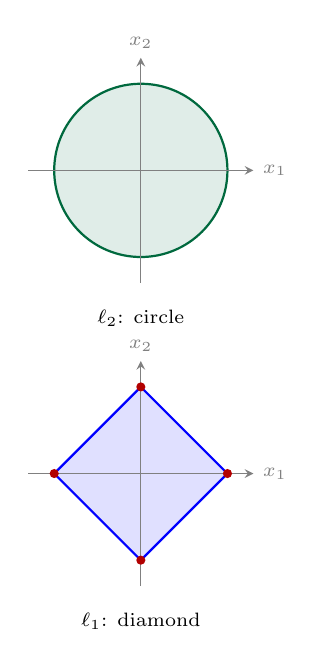
\begin{tikzpicture}[>=stealth, scale=1.1]
\begin{scope}[shift={(0,0)}]
    \fill[mantis!12] (0,0) circle (1);
    \draw[thick, mantis] (0,0) circle (1);
    \draw[->, thin, gray] (-1.3,0) -- (1.3,0) node[right, font=\scriptsize] {$x_1$};
    \draw[->, thin, gray] (0,-1.3) -- (0,1.3) node[above, font=\scriptsize] {$x_2$};
    \node[below, font=\scriptsize] at (0,-1.5) {$\ell_2$: circle};
\end{scope}
\begin{scope}[shift={(0,-3.5)}]
    \fill[blue!12] (1,0) -- (0,1) -- (-1,0) -- (0,-1) -- cycle;
    \draw[thick, blue] (1,0) -- (0,1) -- (-1,0) -- (0,-1) -- cycle;
    \draw[->, thin, gray] (-1.3,0) -- (1.3,0) node[right, font=\scriptsize] {$x_1$};
    \draw[->, thin, gray] (0,-1.3) -- (0,1.3) node[above, font=\scriptsize] {$x_2$};
    \fill[red!70!black] (1,0) circle (1.5pt);
    \fill[red!70!black] (0,1) circle (1.5pt);
    \fill[red!70!black] (-1,0) circle (1.5pt);
    \fill[red!70!black] (0,-1) circle (1.5pt);
    \node[below, font=\scriptsize] at (0,-1.5) {$\ell_1$: diamond};
\end{scope}
\end{tikzpicture}
\end{center}
\end{columns}

\end{frame}

% ------------------------------------------------------------------
\begin{frame}{Rank, Determinant, and Invertibility}

\begin{itemize}
  \item \textbf{Rank:} dimension of the image $\{\mathbf{A}\mathbf{x}\}$; counts independent columns
  \item \textbf{Null space:} $\ker(\mathbf{A}) = \{\mathbf{x} : \mathbf{A}\mathbf{x} = \mathbf{0}\}$; directions lost by the map
  \item \textbf{Determinant:} the factor by which $\mathbf{A}$ scales areas/volumes
\end{itemize}

\bigskip

\begin{block}{Invertibility}
$\mathbf{A}$ is invertible $\iff$ $\det(\mathbf{A}) \neq 0$ $\iff$ $\rank(\mathbf{A}) = d$ $\iff$ $\ker(\mathbf{A}) = \{\mathbf{0}\}$.
\end{block}

\bigskip

\begin{itemize}
  \item $\det(\mathbf{A}) = 0$: columns are dependent, parallelogram collapses
  \item $\det(\mathbf{A}\mathbf{B}) = \det(\mathbf{A})\det(\mathbf{B})$; \quad $\det(\mathbf{A}) = \prod_j\lambda_j$
  \item For OLS: $\mathbf{X}^\top\mathbf{X}$ must be invertible $\Rightarrow$ need $\rank(\mathbf{X}) = d$, so $n \geq d$
\end{itemize}

\end{frame}

% ------------------------------------------------------------------
\begin{frame}{Positive Definiteness}

$\mathbf{A} \succ 0$ means $\mathbf{v}^\top\mathbf{A}\mathbf{v} > 0$ for all $\mathbf{v} \neq \mathbf{0}$.

\bigskip

\textbf{Geometric meaning:} the angle between $\mathbf{v}$ and $\mathbf{A}\mathbf{v}$ is always acute.

\begin{center}
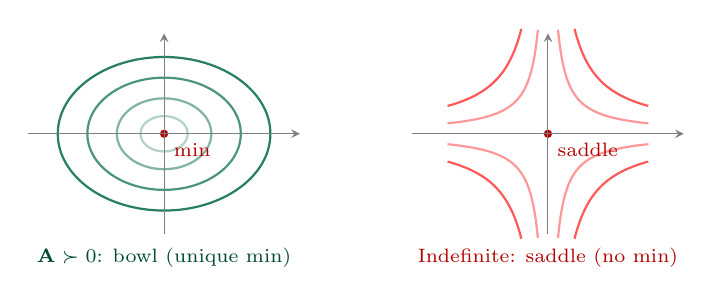
\begin{tikzpicture}[>=stealth, scale=0.75]
\begin{scope}[shift={(0,0)}]
    \draw[mantis!30, thick] (0,0) ellipse (0.4 and 0.3);
    \draw[mantis!50, thick] (0,0) ellipse (0.8 and 0.6);
    \draw[mantis!70, thick] (0,0) ellipse (1.3 and 0.95);
    \draw[mantis!85, thick] (0,0) ellipse (1.8 and 1.3);
    \fill[red!70!black] (0,0) circle (2pt) node[below right, font=\scriptsize] {min};
    \draw[->, thin, gray] (-2.3,0) -- (2.3,0);
    \draw[->, thin, gray] (0,-1.7) -- (0,1.7);
    \node[font=\scriptsize, mantis!70!black] at (0, -2.1) {$\mathbf{A} \succ 0$: bowl (unique min)};
\end{scope}
\begin{scope}[shift={(6.5,0)}]
    \draw[red!40, thick] plot[domain=0.17:1.7, samples=50, smooth] (\x, {0.3/\x});
    \draw[red!40, thick] plot[domain=-1.7:-0.17, samples=50, smooth] (\x, {0.3/\x});
    \draw[red!40, thick] plot[domain=0.17:1.7, samples=50, smooth] (\x, {-0.3/\x});
    \draw[red!40, thick] plot[domain=-1.7:-0.17, samples=50, smooth] (\x, {-0.3/\x});
    \draw[red!65, thick] plot[domain=0.45:1.7, samples=50, smooth] (\x, {0.8/\x});
    \draw[red!65, thick] plot[domain=-1.7:-0.45, samples=50, smooth] (\x, {0.8/\x});
    \draw[red!65, thick] plot[domain=0.45:1.7, samples=50, smooth] (\x, {-0.8/\x});
    \draw[red!65, thick] plot[domain=-1.7:-0.45, samples=50, smooth] (\x, {-0.8/\x});
    \fill[red!70!black] (0,0) circle (2pt) node[below right, font=\scriptsize] {saddle};
    \draw[->, thin, gray] (-2.3,0) -- (2.3,0);
    \draw[->, thin, gray] (0,-1.7) -- (0,1.7);
    \node[font=\scriptsize, red!70!black] at (0, -2.1) {Indefinite: saddle (no min)};
\end{scope}
\end{tikzpicture}
\end{center}

\begin{itemize}
  \item PD $\iff$ all eigenvalues $> 0$; \; PSD $\iff$ all eigenvalues $\geq 0$
  \item Hessian of OLS is $\tfrac{2}{n}\mathbf{X}^\top\mathbf{X} \succeq 0$ $\Rightarrow$ loss surface is a bowl
\end{itemize}

\end{frame}

% ------------------------------------------------------------------
\begin{frame}{Orthogonal Projection}

The \textbf{orthogonal projection} of $\mathbf{y}$ onto subspace $V$ is the closest point $\hat{\mathbf{y}} \in V$.

\begin{center}
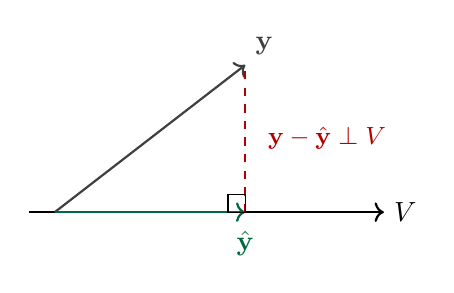
\begin{tikzpicture}[scale=1.1]
    \draw[->, thick] (-0.3,0) -- (3.8,0) node[right] {$V$};
    \draw[->, color=mantis, thick] (0,0) -- (2.2, 0) node[below, yshift=-3pt] {$\hat{\mathbf{y}}$};
    \draw[->, color=darkgray, thick] (0,0) -- (2.2, 1.7) node[above right] {$\mathbf{y}$};
    \draw[dashed, color=red!70!black, thick] (2.2,0) -- (2.2, 1.7);
    \node[right, color=red!70!black, font=\small] at (2.35, 0.85) {$\mathbf{y} - \hat{\mathbf{y}} \perp V$};
    \draw (2.0,0) rectangle (2.2, 0.2);
\end{tikzpicture}
\end{center}

\begin{itemize}
  \item The residual $\mathbf{y} - \hat{\mathbf{y}}$ is $\perp$ to every vector in $V$
  \item The shortest path from a point to a plane always hits at a right angle
\end{itemize}

\bigskip

\begin{alertblock}{Connection to OLS}
$\hat{\mathbf{y}} = \mathbf{X}\hat{\bm{\theta}}$ is the projection of $\mathbf{y}$ onto $\text{Im}(\mathbf{X})$. The normal equations $\mathbf{X}^\top(\mathbf{y} - \mathbf{X}\hat{\bm{\theta}}) = \mathbf{0}$ say residuals $\perp$ columns of $\mathbf{X}$.
\end{alertblock}

\end{frame}

% ==================================================================
\section{Probability}
% ==================================================================

% ------------------------------------------------------------------
\begin{frame}{From Counting to Density}

\textbf{Discrete:} $P(A) = |A|/|\Omega|$ (count favorable / total).

\bigskip

\textbf{Continuous:} $P(X = x) = 0$ for every $x$, so we replace counting with \textbf{density}:
$$P(a \leq X \leq b) = \int_a^b f(x)\,dx$$

\bigskip

\begin{itemize}
  \item $f(x)$ is probability per unit length, \textbf{not} a probability itself (can exceed 1)
  \item What must equal 1 is the total integral: $\int_{-\infty}^{\infty} f(x)\,dx = 1$
  \item \textbf{CDF:} $F(x) = P(X \leq x) = \int_{-\infty}^{x} f(t)\,dt$
  \item $f(x) = F'(x)$: the PDF is the derivative of the CDF
\end{itemize}

\end{frame}

% ------------------------------------------------------------------
\begin{frame}{Expectation, Variance, Covariance}

\textbf{Expectation} (density-weighted average):
$$\E[X] = \int x\,f(x)\,dx \qquad \text{Linearity: } \E[aX + bY] = a\E[X] + b\E[Y]$$

\textbf{Variance:} $\Var(X) = \E[(X - \E[X])^2] = \E[X^2] - (\E[X])^2$

\bigskip

\textbf{Covariance:} $\Cov(X,Y) = \E[XY] - \E[X]\E[Y]$

\smallskip

\textbf{Correlation:} $\rho_{X,Y} = \Cov(X,Y)/(\sigma_X\sigma_Y) \in [-1,1]$

\bigskip

\begin{block}{Key Properties}
\begin{itemize}
  \item $\Var(aX + b) = a^2\Var(X)$
  \item $\Var(X+Y) = \Var(X) + \Var(Y) + 2\Cov(X,Y)$
  \item $\Cov(X,Y) = 0 \not\Rightarrow$ independence (only linear dependence is measured)
\end{itemize}
\end{block}

\end{frame}

% ------------------------------------------------------------------
\begin{frame}{The Covariance Matrix}

For $\mathbf{X} \in \R^d$:
$$\bm{\Sigma} = \E[(\mathbf{X} - \E[\mathbf{X}])(\mathbf{X} - \E[\mathbf{X}])^\top] \in \R^{d \times d}$$

\begin{itemize}
  \item Diagonal entries $\Sigma_{ii} = \sigma_i^2$; off-diagonal $\Sigma_{ij} = \rho_{ij}\sigma_i\sigma_j$
  \item Always PSD: $\mathbf{v}^\top\bm{\Sigma}\mathbf{v} = \E[(\mathbf{v}^\top(\mathbf{X} - \bm{\mu}))^2] \geq 0$
  \item Linear transformation: $\Var(\mathbf{A}\mathbf{X}) = \mathbf{A}\bm{\Sigma}\mathbf{A}^\top$
\end{itemize}

\bigskip

\begin{block}{Whitening}
The Cholesky factorization $\bm{\Sigma} = \mathbf{L}\mathbf{L}^\top$ is the multivariate ``square root.'' The whitening transform $\mathbf{Z} = \mathbf{L}^{-1}(\mathbf{X} - \bm{\mu})$ gives $\Var(\mathbf{Z}) = \mathbf{I}$ (multivariate $z$-score).
\end{block}

\end{frame}

% ------------------------------------------------------------------
\begin{frame}{Key Distributions}

\textbf{Bernoulli}$(\pi)$: $P(X\!=\!1) = \pi$, building block for logistic regression.

\bigskip

\textbf{Gaussian} $\mathcal{N}(\mu, \sigma^2)$:
$$f(x) = \frac{1}{\sqrt{2\pi\sigma^2}}\exp\!\left(-\frac{(x - \mu)^2}{2\sigma^2}\right)$$

\begin{center}
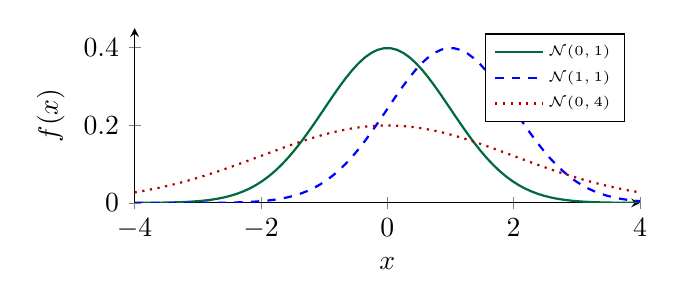
\begin{tikzpicture}
\begin{axis}[
    width=8cm, height=3.8cm,
    xlabel={$x$}, ylabel={$f(x)$},
    xmin=-4, xmax=4, ymin=0, ymax=0.45,
    axis lines=left,
    legend style={font=\tiny, at={(0.97,0.97)}, anchor=north east},
    grid=none,
]
\addplot[domain=-4:4, samples=80, color=mantis, thick] {exp(-x^2/2)/sqrt(2*3.14159)};
\addplot[domain=-4:4, samples=80, color=blue, thick, dashed] {exp(-(x-1)^2/2)/sqrt(2*3.14159)};
\addplot[domain=-4:4, samples=80, color=red!70!black, thick, dotted] {exp(-x^2/8)/sqrt(8*3.14159)};
\legend{{$\mathcal{N}(0,1)$}, {$\mathcal{N}(1,1)$}, {$\mathcal{N}(0,4)$}}
\end{axis}
\end{tikzpicture}
\end{center}

Minimizing squared error $=$ maximizing Gaussian log-likelihood. Linear combos of independent Gaussians are Gaussian.

\end{frame}

% ------------------------------------------------------------------
\begin{frame}{Independence and the CLT}

\textbf{Independence:} $P(X \in A,\, Y \in B) = P(X \in A)\,P(Y \in B)$ for all $A, B$.

\textbf{i.i.d.:} mutually independent and same distribution (standing assumption for training data).

\bigskip

\textbf{Conditional expectation:} $\E[Y \mid X = x]$ is the best predictor under squared loss.

\begin{itemize}
  \item Law of Total Expectation: $\E[Y] = \E_X[\E[Y \mid X]]$
  \item Law of Total Variance: $\Var(Y) = \E_X[\Var(Y \mid X)] + \Var_X(\E[Y \mid X])$
\end{itemize}

\bigskip

\begin{block}{Central Limit Theorem (De Moivre--Laplace)}
As $n \to \infty$, standardized Binomial $\to$ Normal:
$$\frac{X - n\pi}{\sqrt{n\pi(1-\pi)}} \xrightarrow{d} \mathcal{N}(0, 1)$$
\end{block}

\end{frame}

% ==================================================================
\section{Statistics}
% ==================================================================

% ------------------------------------------------------------------
\begin{frame}{Estimators: Bias, Variance, MSE}

$\hat{\theta} = g(X_1, \ldots, X_n)$ estimates unknown $\theta$ from i.i.d.\ data.

\bigskip

\begin{itemize}
  \item \textbf{Bias:} $\Bias(\hat{\theta}) = \E[\hat{\theta}] - \theta$; unbiased if $\E[\hat{\theta}] = \theta$
  \item \textbf{Variance:} $\Var(\hat{\theta})$; fluctuation across samples
\end{itemize}

\bigskip

\begin{block}{MSE Decomposition}
$$\MSE(\hat{\theta}) = \E[(\hat{\theta} - \theta)^2] = \Bias(\hat{\theta})^2 + \Var(\hat{\theta})$$
\end{block}

\bigskip

A \textbf{biased} estimator with low variance (Ridge) can have lower MSE than an \textbf{unbiased} one with high variance (OLS in high dimensions).

\end{frame}

% ------------------------------------------------------------------
\begin{frame}{Maximum Likelihood Estimation}

Given i.i.d.\ data from $p(x; \theta)$, the \textbf{log-likelihood}:
$$\ell(\theta) = \sum_{i=1}^{n} \log p(x_i; \theta) \qquad \hat{\theta}_{\text{MLE}} = \arg\max_\theta\,\ell(\theta)$$

\bigskip

\textbf{Gaussian mean:} $\ell(\mu) = \text{const} - \frac{1}{2\sigma^2}\sum(x_i - \mu)^2$ $\Rightarrow$ $\hat{\mu} = \bar{x}$.

Minimizing squared error $=$ Gaussian MLE $\Rightarrow$ OLS is MLE under Gaussian noise.

\bigskip

\textbf{Bernoulli:} $\hat{\pi} = \bar{x}$ (sample proportion). Logistic regression extends this by letting $\pi$ depend on $\mathbf{x}$ through a sigmoid.

\bigskip

\begin{block}{Asymptotic Properties}
MLE is \textbf{consistent}, \textbf{asymptotically normal}, and \textbf{efficient} (achieves the Cram\'er--Rao bound).
\end{block}

\end{frame}

% ==================================================================
\section{The Learning Problem}
% ==================================================================

% ------------------------------------------------------------------
\begin{frame}{Supervised Learning and ERM}

Training set $D_n = \{(x_i, y_i)\}_{i=1}^n \sim \nu^n$. Goal: predict $y$ on unseen $x$.

\begin{itemize}
  \item \textbf{Regression:} $\mathcal{Y} = \R$ \quad \textbf{Classification:} $\mathcal{Y} = \{0,1,\ldots,K\}$
\end{itemize}

\bigskip

\textbf{True risk:} $\mathcal{R}(f) = \E_{(x,y)\sim\nu}[\ell(y, f(x))]$ (unknown $\nu$)

\textbf{Empirical risk:} $\hat{\mathcal{R}}_n(f) = \frac{1}{n}\sum_{i=1}^{n}\ell(y_i, f(x_i))$

\bigskip

\begin{block}{Empirical Risk Minimization}
$$\hat{f} = \arg\min_{f \in \mathcal{F}}\;\hat{\mathcal{R}}_n(f)$$
The gap $\mathcal{R}(\hat{f}) - \hat{\mathcal{R}}_n(\hat{f})$ is the \textbf{generalization gap}.
\end{block}

\bigskip

\textbf{Bayes optimal:} $f^*(x) = \E[y \mid x]$ under squared loss. Error decomposes as:
$\mathcal{R}(\hat{f}) = \underbrace{\mathcal{R}^*}_{\text{irreducible}} + \underbrace{\Bias^2 + \Var}_{\text{reducible}}$

\end{frame}

% ------------------------------------------------------------------
\begin{frame}{Loss Functions}

\begin{center}
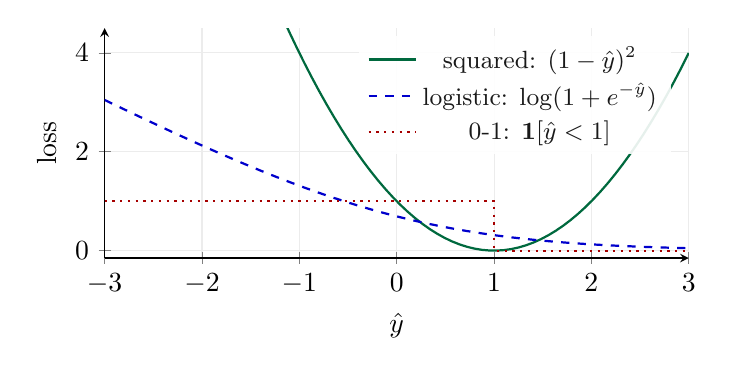
\begin{tikzpicture}
\begin{axis}[
    width=9cm, height=4.5cm,
    xlabel={$\hat{y}$}, ylabel={loss},
    xmin=-3, xmax=3, ymin=-0.15, ymax=4.5,
    axis lines=left,
    grid=major, grid style={gray!15},
    legend style={at={(0.97,0.97)}, anchor=north east, font=\small, draw=none, fill=white, fill opacity=0.9},
]
\addplot[domain=-3:3, samples=80, color=mantis, thick] {(1 - x)^2};
\addlegendentry{squared: $(1-\hat{y})^2$}
\addplot[domain=-3:3, samples=80, color=blue!80!black, thick, dashed] {ln(1 + exp(-x))};
\addlegendentry{logistic: $\log(1+e^{-\hat{y}})$}
\addplot[color=red!65!black, thick, dotted] coordinates {(-3,1) (1,1) (1,0) (3,0)};
\addlegendentry{0-1: $\mathbf{1}[\hat{y}<1]$}
\end{axis}
\end{tikzpicture}
\end{center}

\begin{itemize}
  \item \textbf{Squared:} convex, differentiable; sensitive to outliers
  \item \textbf{0-1:} non-convex, non-differentiable; NP-hard to minimize
  \item \textbf{Logistic / Cross-entropy:} convex surrogate for 0-1 loss; penalizes confident wrong predictions heavily
  \item Convex loss $\Rightarrow$ local min = global min $\Rightarrow$ gradient descent converges
\end{itemize}

\end{frame}

% ------------------------------------------------------------------
\begin{frame}{Generative vs.\ Discriminative Models}

The joint distribution factorizes in two ways:
$$p(x, y) = \underbrace{p(y \mid x)}_{\text{discriminative}} \cdot p(x) = \underbrace{p(x \mid y)}_{\text{generative}} \cdot p(y)$$

\bigskip

\begin{columns}[t]
\column{0.48\textwidth}
\begin{block}{Discriminative}
Model $p(y \mid x)$ directly.

\smallskip
Examples: linear regression, logistic regression, neural networks.

\smallskip
Better with large $n$; only models what's needed for prediction.
\end{block}

\column{0.48\textwidth}
\begin{block}{Generative}
Model $p(x \mid y)$ and $p(y)$, use Bayes' rule.

\smallskip
Examples: GDA, Naive Bayes.

\smallskip
Stronger assumptions; more data-efficient when assumptions hold.
\end{block}
\end{columns}

\end{frame}

% ==================================================================
\section{Summary}
% ==================================================================

% ------------------------------------------------------------------
\begin{frame}{Recap: The Full Picture}

\begin{enumerate}
  \item \textbf{Calculus:} derivatives, chain rule (backprop), gradients (gradient descent), convexity (unique solutions).
  \item \textbf{Linear algebra:} matrices as transformations, dot products, norms ($\ell_1$ vs $\ell_2$ for regularization), PSD (bowl-shaped loss), projection (OLS geometry).
  \item \textbf{Probability:} density, expectation, variance, covariance matrix, key distributions, CLT.
  \item \textbf{Statistics:} bias-variance tradeoff, MLE (OLS $=$ Gaussian MLE).
  \item \textbf{Learning:} ERM, generalization gap, Bayes optimal predictor, loss functions, generative vs.\ discriminative.
\end{enumerate}

\end{frame}

% ------------------------------------------------------------------
{
\setbeamercolor{background canvas}{bg=mantis}
\setbeamercolor{normal text}{fg=white}
\usebeamercolor[fg]{normal text}
\begin{frame}[c]
\centering
\Huge\textbf{Questions?}
\end{frame}
}

\end{document}
